\documentclass{article}
\usepackage[dvipsnames]{xcolor}
\usepackage[utf8]{inputenc}
\usepackage{appendix}
\usepackage[T1]{fontenc}
\usepackage[italian]{babel}
\usepackage{siunitx} % Provides the \SI{}{} and \si{} command for typesetting SI units
\usepackage{graphicx} % Required for the inclusion of images
\usepackage{natbib} % Required to change bibliography style to APA
\usepackage{amsmath} % Required for some math elements
\usepackage{caption}
\usepackage{float}
\usepackage{import}
\setlength\parindent{0pt} % Removes all indentation from paragraphs
\usepackage{minted}

\usepackage{tikz}
\usetikzlibrary{arrows,shadows}
\usepackage{pgf-umlsd}
\usepackage{wrapfig}

\title{\vspace{-2cm}Progetto di Tecnologie Informatiche per il Web} % Title
\author{Negri Riccardo} % Author name
\date{\today}


\begin{document}

\maketitle

\begin{figure}[H]
\centering
\includegraphics[width=0.365\textwidth]{assets/logo.jpg}
\end{figure}

\begin{center}
\begin{tabular}{l l l l}
Docente: & Fraternali Piero& & \\ 
Studente: & Negri Riccardo & 10729927 & 936820 
\end{tabular}
\end{center}

\tableofcontents
\pagebreak

\section{Specifiche}

\subsection{Versione pure HTML}
Un’applicazione web consente la gestione di trasferimenti di denaro online da un conto a un
altro. L’applicazione supporta registrazione e login mediante una pagina pubblica con
opportune form. La registrazione controlla la validità sintattica dell’indirizzo di email e
l’uguaglianza tra i campi “password” e “ripeti password”. La registrazione controlla l’unicità
dello username. Un utente ha un nome, un cognome, uno username e uno o più conti correnti.
Un conto ha un codice, un saldo, e i trasferimenti fatti (in uscita) e ricevuti (in ingresso) dal
conto. Un trasferimento ha una data, un importo, un conto di origine e un conto di destinazione.
Quando l’utente accede all’applicazione appare una pagina LOGIN per la verifica delle
credenziali. In seguito all’autenticazione dell’utente appare l’HOME page che mostra l’elenco
dei suoi conti. Quando l’utente seleziona un conto, appare una pagina STATO DEL CONTO
che mostra i dettagli del conto e la lista dei movimenti in entrata e in uscita, ordinati per data
discendente. La pagina contiene anche una form per ordinare un trasferimento. La form
contiene i campi: codice utente destinatario, codice conto destinatario, causale e importo.
All’invio della form con il bottone INVIA, l’applicazione controlla che il conto di destinazione
appartenga all’utente specificato e che il conto origine abbia un saldo superiore o uguale
all’importo del trasferimento. In caso di mancanza di anche solo una condizione, l’applicazione
mostra una pagina con un avviso di fallimento che spiega il motivo del mancato trasferimento.
Nel caso in cui entrambe le condizioni siano soddisfatte, l’applicazione deduce l’importo dal
conto di origine, aggiunge l’importo al conto di destinazione e mostra una pagina CONFERMA
TRASFERIMENTO che presenta i dati dell’importo trasferito e i dati del conto di origine e di
destinazione con i rispettivi saldi precedenti al trasferimento e aggiornati dopo il trasferimento.
L’applicazione deve garantire l’atomicità del trasferimento: ogni volta che il conto di
destinazione viene addebitato, il conto di origine deve essere accreditato. Ogni pagina
contiene un collegamento per tornare alla pagina precedente. L’applicazione consente il
logout dell’utente.

\pagebreak
\subsection{Versione RIA}
Si realizzi un’applicazione client server web che modifica le specifiche precedenti come segue:
\begin{itemize}
\item La registrazione controlla la validità sintattica dell’indirizzo di email e l’uguaglianza tra
i campi “password” e “ripeti password”, anche a lato client.
\item Dopo il login, l’intera applicazione è realizzata con un’unica pagina.
\item 	Ogni interazione dell’utente è gestita senza ricaricare completamente la pagina, ma
produce l’invocazione asincrona del server e l’eventuale modifica del contenuto da
aggiornare a seguito dell’evento.
\item I controlli di validità dei dati di input (ad esempio importo non nullo e maggiore di zero)
devono essere realizzati anche a lato client.
\item L’avviso di fallimento è realizzato mediante un messaggio nella pagina che ospita
l’applicazione.
\item L’applicazione chiede all’utente se vuole inserire nella propria rubrica i dati del
destinatario di un trasferimento andato a buon fine non ancora presente. Se l’utente
conferma, i dati sono memorizzati nella base di dati e usati per semplificare
l’inserimento. Quando l’utente crea un trasferimento, l’applicazione propone mediante
una funzione di auto-completamento i destinatari in rubrica il cui codice corrisponde
alle lettere inserite nel campo codice utente destinatario.
\end{itemize}

\pagebreak
\section{Database design}

\subsection{Analisi testo delle specifiche}
Legenda: \textcolor{red}{entità}, \textcolor{ForestGreen}{attributi}, \textcolor{blue}{relazioni}.
\\
\\
Un’applicazione web consente la gestione di trasferimenti di denaro online da un conto a un
altro. L’applicazione supporta registrazione e login mediante una pagina pubblica con
opportune form. La registrazione controlla la validità sintattica dell’\textcolor{ForestGreen}{indirizzo di email} e
l’uguaglianza tra i campi “\textcolor{ForestGreen}{password}” e “ripeti password”. La registrazione controlla l’unicità
dello username. Un \textcolor{red}{utente} ha un \textcolor{ForestGreen}{nome}, un \textcolor{ForestGreen}{cognome}, uno \textcolor{ForestGreen}{username} e \textcolor{blue}{uno o più conti correnti}.
Un \textcolor{red}{conto}  ha un \textcolor{ForestGreen}{codice}, un \textcolor{ForestGreen}{saldo}, e i \textcolor{blue}{trasferimenti fatti (in uscita) e ricevuti (in ingresso)} dal
conto. Un  \textcolor{red}{trasferimento} ha una \textcolor{ForestGreen}{data}, un \textcolor{ForestGreen}{importo}, un \textcolor{blue}{conto di origine e un conto di destinazione}.
Quando l’utente accede all’applicazione appare una pagina LOGIN per la verifica delle
credenziali. In seguito all’autenticazione dell’utente appare l’HOME page che mostra l’elenco
dei suoi conti. Quando l’utente seleziona un conto, appare una pagina STATO DEL CONTO
che mostra i dettagli del conto e la lista dei movimenti in entrata e in uscita, ordinati per data
discendente. La pagina contiene anche una form per ordinare un trasferimento. La form
contiene i campi: codice utente destinatario, codice conto destinatario, \textcolor{ForestGreen}{causale} e importo.
All’invio della form con il bottone INVIA, l’applicazione controlla che il conto di destinazione
appartenga all’utente specificato e che il conto origine abbia un saldo superiore o uguale
all’importo del trasferimento. In caso di mancanza di anche solo una condizione, l’applicazione
mostra una pagina con un avviso di fallimento che spiega il motivo del mancato trasferimento.
Nel caso in cui entrambe le condizioni siano soddisfatte, l’applicazione deduce l’importo dal
conto di origine, aggiunge l’importo al conto di destinazione e mostra una pagina CONFERMA
TRASFERIMENTO che presenta i dati dell’importo trasferito e i dati del conto di origine e di
destinazione con i rispettivi saldi precedenti al trasferimento e aggiornati dopo il trasferimento.
L’applicazione deve garantire l’atomicità del trasferimento: ogni volta che il conto di
destinazione viene addebitato, il conto di origine deve essere accreditato. Ogni pagina
contiene un collegamento per tornare alla pagina precedente. L’applicazione consente il
logout dell’utente.
\\
\\
Si realizzi un’applicazione client server web che modifica le specifiche precedenti come segue:
\begin{itemize}
\item La registrazione controlla la validità sintattica dell’indirizzo di email e l’uguaglianza tra
i campi “password” e “ripeti password”, anche a lato client.
\item Dopo il login, l’intera applicazione è realizzata con un’unica pagina.
\item 	Ogni interazione dell’utente è gestita senza ricaricare completamente la pagina, ma
produce l’invocazione asincrona del server e l’eventuale modifica del contenuto da
aggiornare a seguito dell’evento.
\item I controlli di validità dei dati di input (ad esempio importo non nullo e maggiore di zero)
devono essere realizzati anche a lato client.
\item L’avviso di fallimento è realizzato mediante un messaggio nella pagina che ospita
l’applicazione.
\item L’applicazione chiede all’utente se vuole  \textcolor{blue}{inserire nella propria rubrica i dati del
destinatario} di un trasferimento andato a buon fine non ancora presente. Se l’utente
conferma, i dati sono memorizzati nella base di dati e usati per semplificare
l’inserimento. Quando l’utente crea un trasferimento, l’applicazione propone mediante
una funzione di auto-completamento i destinatari in rubrica il cui codice corrisponde
alle lettere inserite nel campo codice utente destinatario.
\end{itemize}

\subsection{Progetto concettuale - Diagramma E-R (Entità-Relazione)}
\begin{figure}[H]
\centering
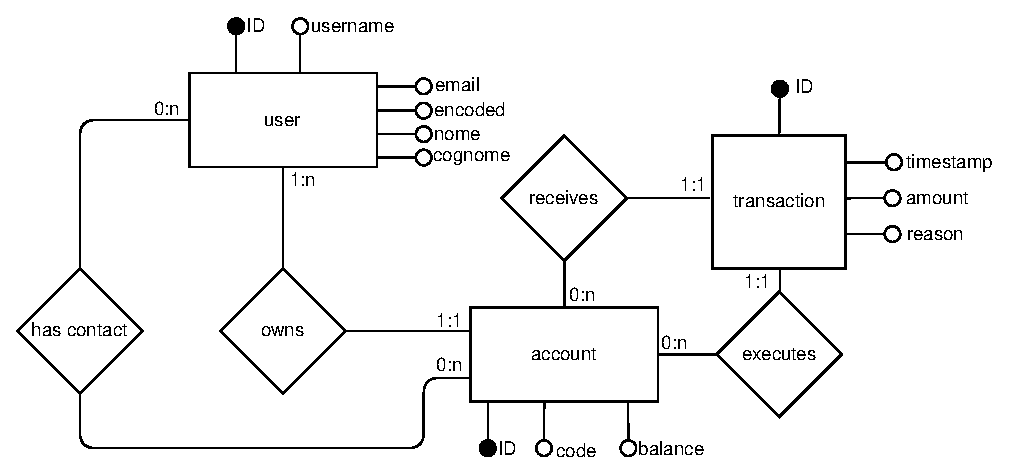
\includegraphics[width=1\textwidth]{assets/diagram.eps}
\end{figure}

\subsection{Progetto logico}
USER(\underline{ID}, username, email, encoded, name, surname)
\\
ACCOUNT(\underline{ID}, code, balance, user)
\\
TRANSACTION(\underline{ID}, timestamp, amount, reason, origin, destination)
\\
CONTACT(\underline{owner}, \underline{element})

\subsection{Database schema}
Nel db tutti gli on delete sono no action perché ho la necessità di mantenere le informazioni per il futuro (da argomentare meglio)

Statement per creare il database:
\begin{minted}{mysql}
CREATE DATABASE tiw_db;
\end{minted}

Statements per creare le tabelle: 
\begin{minted}{mysql}
CREATE TABLE `tiw_db`.`user` (
`id` INT NOT NULL AUTO_INCREMENT,
`username` VARCHAR(45) NOT NULL UNIQUE,
`email` VARCHAR(45) NOT NULL UNIQUE,
`encoded` VARCHAR(255) NOT NULL,
`name` VARCHAR(45) NOT NULL,
`surname` VARCHAR(45) NOT NULL,
PRIMARY KEY (`id`)
);
\end{minted}

\begin{minted}{mysql}
CREATE TABLE `tiw_db`.`account` (
`id` INT NOT NULL AUTO_INCREMENT,
`code` CHAR(12) NOT NULL UNIQUE,
`balance` FLOAT NOT NULL DEFAULT 0,
`user` INT NOT NULL,
PRIMARY KEY (`id`),
CONSTRAINT `user_account` FOREIGN KEY (`user`) 
REFERENCES `tiw_db`.`user` (`id`) 
ON DELETE NO ACTION ON UPDATE CASCADE
);
\end{minted}

\begin{minted}{mysql}
CREATE TABLE `tiw_db`.`transaction` (
`id` INT NOT NULL AUTO_INCREMENT,
`timestamp` DATETIME DEFAULT CURRENT_TIMESTAMP,
`amount` FLOAT NOT NULL,
`reason` VARCHAR(255) NOT NULL,
`origin` INT NOT NULL,
`destination` INT NOT NULL,
PRIMARY KEY (`id`),
CONSTRAINT `transaction_origin` FOREIGN KEY (`origin`) 
REFERENCES `tiw_db`.`account` (`id`)
ON DELETE NO ACTION ON UPDATE CASCADE,
CONSTRAINT `transaction_destination` FOREIGN KEY (`destination`) 
REFERENCES `tiw_db`.`account` (`id`) 
ON DELETE NO ACTION ON UPDATE CASCADE
);
\end{minted}
\pagebreak

\begin{minted}{mysql}
CREATE TABLE `tiw_db`.`contact` (
`owner` INT,
`element` INT,
PRIMARY KEY (`owner`, `element`),
CONSTRAINT `contact_owner` FOREIGN KEY (`owner`) 
REFERENCES `tiw_db`.`user` (`id`)
ON DELETE NO ACTION ON UPDATE CASCADE,
CONSTRAINT `contact_element` FOREIGN KEY (`element`) 
REFERENCES `tiw_db`.`account` (`id`) 
ON DELETE NO ACTION ON UPDATE CASCADE
);
\end{minted}

\subsection{Hashing della password}
Si è deciso di usare Argon2 come algoritmo di hash delle password. Argon2 applica una funzione pseudocasuale alla password o passphrase di input insieme a un valore \texttt{salt} e ripete il processo molte volte per produrre una chiave derivata, che può quindi essere utilizzata come chiave crittografica nelle operazioni successive. Il lavoro di calcolo aggiunto rende molto più difficile il cracking delle password ed è noto come \texttt{key stretching}. Infatti è volutamente dispendioso in termini computazionali.
\\\\
Il motivo per cui si utilizza un \texttt{salt} durante l'hashing delle password è che randomizzano l'hash generato per lo stesso valore di input. Quindi, se due utenti hanno la stessa password, i loro hash saranno comunque diversi. Ciò rallenterà ulteriormente il processo di decifrazione della password da parte di un avversario.
\\
Argon2 genera internamente un nuovo \texttt{salt} per ogni nuova richiesta di generare un hash. Quindi, se si richiede un hash per lo stesso testo in chiaro più volte, ogni volta si ottiene un hash diverso. 
\\ \\
Di seguito un esempio di come viene salvata nel database l'informazione necessaria per verificare la password di un utente:\\ \texttt{\$argon2i\$v=19\$m=65536,t=10,p=1\$PCMn0NBsYymo2jJIeoVwsA\$rmrwpTVQks5s\\LsUKBfImzV9/b0HwF9hZKe1b5dQWwYo}
\\
Analisi dei valori:
\begin{itemize}
\item \texttt{argon2i} indica la  variante di Argon2 in uso;
\item \texttt{v=19} indica la versione di Argon;
\item \texttt{m=65536} indica l'utilizzo di memoria;
\item \texttt{t=10} indica le iterazioni;
\item \texttt{p=1} indica il numero di thread da utilizzare;
\item \texttt{PCMn0NBsYymo2jJIeoVwsA} è il \texttt{salt} di 16 byte;
\item \texttt{rmrwpTVQks5sLsUKBfImzV9/b0HwF9hZKe1b5dQWwYo} è l'\texttt{hash} di 32 byte.
\end{itemize}
Sul computer in uso al momento la validazione di una password rispetto all'\texttt{encoded} sopra ripotato impiega circa 400ms. 

\subsection{Script Python per popolare il database}
Al fine di popolare automaticamente un nuovo database è stato creato uno script in Python chiamato "populate-tiw-db.py" .

\section{Versione pure HTML}

\subsection{Analisi requisiti delle specifiche}
Legenda: \textcolor{red}{pagine}, \textcolor{ForestGreen}{view components}, \textcolor{blue}{eventi}, \textcolor{brown}{azioni}.
\\
\\
Un’applicazione web consente la gestione di trasferimenti di denaro online da un conto a un
altro. L’applicazione supporta  \textcolor{brown}{registrazione} e  \textcolor{blue}{login} mediante una pagina pubblica con
opportune  \textcolor{ForestGreen}{form}. La registrazione controlla la validità sintattica dell’indirizzo di email e
l’uguaglianza tra i campi “password” e “ripeti password”. La registrazione controlla l’unicità
dello username. Un utente ha un nome, un cognome, uno username e uno o più conti correnti.
Un conto ha un codice, un saldo, e i trasferimenti fatti (in uscita) e ricevuti (in ingresso) dal
conto. Un trasferimento ha una data, un importo, un conto di origine e un conto di destinazione.
Quando l’utente accede all’applicazione appare una  \textcolor{red}{pagina LOGIN} per la verifica delle
credenziali. In seguito all’autenticazione dell’utente appare \textcolor{red}{l’HOME page} che \textcolor{ForestGreen}{mostra l’elenco
dei suoi conti}. Quando l’utente  \textcolor{blue}{seleziona un conto}, appare una \textcolor{red}{pagina STATO DEL CONTO}
che mostra i \textcolor{ForestGreen}{dettagli del conto e la lista dei movimenti in entrata e in uscita}, ordinati per data
discendente. La pagina contiene anche una \textcolor{ForestGreen}{form} per ordinare un trasferimento. La form
contiene i campi: codice utente destinatario, codice conto destinatario, causale e importo.
All’invio della form con il bottone INVIA, l’applicazione controlla che il conto di destinazione
appartenga all’utente specificato e che il conto origine abbia un saldo superiore o uguale
all’importo del trasferimento. In caso di mancanza di anche solo una condizione, l’applicazione
mostra una \textcolor{red}{pagina con un avviso di fallimento} che spiega il \textcolor{ForestGreen}{motivo del mancato trasferimento}.
Nel caso in cui entrambe le condizioni siano soddisfatte, l’applicazione \textcolor{brown}{deduce l’importo dal
conto di origine, aggiunge l’importo al conto di destinazione} e mostra una \textcolor{red}{pagina CONFERMA
TRASFERIMENTO} che presenta i \textcolor{ForestGreen}{dati dell’importo trasferito e i dati del conto di origine e di
destinazione con i rispettivi saldi precedenti al trasferimento e aggiornati dopo il trasferimento}.
L’applicazione deve garantire l’atomicità del trasferimento: ogni volta che il conto di
destinazione viene addebitato, il conto di origine deve essere accreditato. Ogni pagina
contiene un \textcolor{ForestGreen}{collegamento per tornare alla pagina precedente}. L’applicazione consente il
\textcolor{blue}{logout} dell’utente.

\subsection{Completamento specifiche}
\begin{itemize}
\item E' stata creata anche una pagina per visualizzare le informazioni dell'utente
\item Si è deciso di implementare la gestione dei contatti e la possibilità di aggiungere un conto ai contatti anche nella versione pure HTML
\item Nella rubrica viene aggiunto solo un conto relativo ad un utente, non tutti i conti di un singolo utente
\item La rubrica è relativa all'utente e non al conto, quindi tutte le pagine dei conti di un utente vedranno la stessa rubrica
\end{itemize}

\subsection{Application Design}
\begin{figure}[H]
	\centering
	\includegraphics[width=1\textwidth]{assets/ifml_pure.png}
\end{figure}

\subsection{Componenti}
\begin{itemize}
	\item Model Objects (Beans)
	\begin{itemize}
		\item Account
		\item Contact
		\item Transaction
		\item User
	\end{itemize}
	\item Data Access Objects (Classes)
	\begin{itemize}
		\item AccountDAO
		\item ContactDAO
		\item TransactionDAO
		\item UserDAO
	\end{itemize}
	\item Controllers (servlets)
	\begin{itemize}
		\item AccountPage
		\item AddContact
		\item ErrorPage
		\item HomePage
		\item Login
		\item Logout
		\item MakeTransaction
		\item ProfilePage
		\item Registration
		\item TransactionOutcomePage
	\end{itemize}
	\item Filters
	\begin{itemize}
		\item AlreadyLoggedInChecker
		\item LoginChecker
	\end{itemize}
	\item Utils
	\begin{itemize}
		\item ConnectionHandler
		\item ParameterValidator
		\item PasswordHashing
	\end{itemize}
	\item Views (Templates)
	\begin{itemize}
		\item account.html
		\item error.html
		\item home.html
		\item login.html
		\item profile.html
		\item registration.html
		\item transaction-outcome.html
	\end{itemize}
	\item Fragments (Templates)
	\begin{itemize}
		\item navbar.html
		\item sidebar.html
	\end{itemize}
\end{itemize}

\subsection{Eventi}
Precisiazioni riguardo ai sequence diagram: con "processed" si intende il file HTML processato tramite \texttt{templateEngine.process()} dopo avere impostato le oppurtune variabili nel \texttt{context}; si assume che le get e le post di seguito rappresentate abbiano già superato i controlli presenti nei filtri.
\subsubsection{Login}
\makebox[\textwidth][c]{
\begin{sequencediagram}
\newinst{client}{Client}
\newinst[5]{login}{Login}
\newinst[4]{dao}{UserDAO}
\begin{call}{client}{doPost(usr, psd)}{login}{redirect to /home}
\begin{call}{login}{validateParameters()}{login}{boolean}
\end{call}
\mess{login}{if false: processed index.html}{client}
\begin{call}{login}{checkUserLogin(usr, psw)}{dao}{user}
\end{call}
\mess{login}{if exception: processed login.html}{client}
\mess{login}{if user === null: processed index.html}{client}
\begin{call}{login}{session.setAttribute(user)}{login}{}
\end{call}
\end{call}
\end{sequencediagram}
}

\subsubsection{Registrazione}
\makebox[\textwidth][c]{
\begin{sequencediagram}
\newinst{client}{Client}
\newinst[5]{reg}{Registration}
\newinst[4]{dao}{UserDAO}
\begin{call}{client}{doPost(usr, email, psw, control, ...)}{reg}{redirect to /login}
\begin{call}{reg}{validateParameters()}{reg}{boolean}
\end{call}
\mess{reg}{if false: processed registration.html}{client}
\begin{call}{reg}{existsUserWithUsername(usr)}{dao}{boolean}
\end{call}
\mess{reg}{if true: processed registration.html}{client}
\begin{call}{reg}{existsUserWithEmail(email)}{dao}{boolean}
\end{call}
\mess{reg}{if true: processed registration.html}{client}
\begin{call}{reg}{createUser(usr, email, psw, ...)}{dao}{boolean}
\end{call}
\mess{reg}{if exception: processed registration.html}{client}
\end{call}
\end{sequencediagram}
}

\subsubsection{Accesso Home Page}
\makebox[\textwidth][c]{
\begin{sequencediagram}
\newinst{client}{Client}
\newinst[5]{home}{HomePage}
\newinst[4]{dao}{AccountDAO}
\begin{call}{client}{doGet()}{home}{processed home.html}
\begin{call}{home}{user = session.getAttribute("user")}{home}{}
\end{call}
\begin{call}{home}{findAccountsWithLastActivity(userId)}{dao}{accounts}
\end{call}
\mess{home}{if exception: sendError}{client}
\end{call}
\end{sequencediagram}
}

\subsubsection{Accesso Account Page}
\makebox[\textwidth][c]{
\begin{sequencediagram}
\newinst{client}{Client}
\newinst[2]{page}{AccountPage}
\newinst[3]{dao1}{AccountDAO}
\newinst{dao2}{ContactDAO}
\begin{call}{client}{doGet()}{page}{processed account.html}
	\begin{call}{page}{user = session.getAttribute("user")}{page}{}
	\end{call}
	\begin{call}{page}{validateParameters()}{page}{}
	\end{call}
	\begin{mess}{page}{if false: sendError}{client}
	\end{mess}
	\begin{call}{page}{checkAccountID()}{page}{}
	\begin{call}{page}{getAccountFromID}{dao1}{account}
	\end{call}
	\end{call}
	\begin{mess}{page}{if not valid: sendError}{client}
	\end{mess}
	\begin{call}{page}{findTransactions(accountID)}{dao1}{accountTransactions}
	\end{call}
	\begin{call}{page}{findContactsFromUserID(userId)}{dao2}{contacts}
	\end{call}
\mess{page}{if exception: sendError}{client}
\end{call}
\end{sequencediagram}
}

\subsubsection{Esegui Transazione}
\makebox[\textwidth][c]{
\begin{sequencediagram}
	\newinst{client}{Client}
	\newinst[2]{make}{MakeTransaction}
	\newinst[1]{dao1}{AccountDAO}
	\newinst{dao2}{UserDAO}
	\newinst{dao3}{TransactionDAO}
	\begin{call}{client}{doPost()}{make}{redirect to /transaction-outcome?id=...}
		\begin{call}{make}{user = session.getAttribute("user")}{make}{}
		\end{call}
	
		\begin{call}{make}{validateParameters()}{make}{}
			\begin{call}{make}{getAccount(originCode)}{dao1}{user}
			\end{call}
		\end{call}
		\mess{make}{if false: sendError}{client}
		\mess{make}{if exception: sendError}{client}
		
		\begin{call}{make}{checkConditions()}{make}{}
			\begin{call}{make}{getAccount(destinationCode)}{dao1}{user}
			\end{call}
		\begin{call}{make}{getUserFromUsername(usr)}{dao2}{user}
		\end{call}
		\end{call}
		\mess{make}{if false: redirect to transaction-outcome?failed=...}{client}
		\mess{make}{if exception: sendError}{client}
		
		\begin{call}{make}{addTransaction(amount, reason, origin, dest)}{dao3}{transactionId}
		\end{call}
		\mess{make}{if exception: sendError}{client}
	\end{call}
\end{sequencediagram}
}

\subsubsection{Esito transazione}
\makebox[\textwidth][c]{
\begin{sequencediagram}
	\newinst{client}{Client}
	\newinst[2]{page}{TransactionOutcomePage}
	\newinst[1]{dao1}{TransactionDAO}
	\newinst{dao2}{AccountDAO}
	\newinst{dao3}{ContactDAO}
	\begin{call}{client}{doGet()}{page}{processed transaction-outcome.html}
		\begin{call}{page}{user = session.getAttribute("user")}{page}{}
		\end{call}
		\begin{call}{page}{validateParameters()}{page}{}
			\begin{call}{page}{getTransaction(id)}{dao1}{transaction}
			\end{call}
		\end{call}
		\mess{page}{if false: sendError}{client}
		\mess{page}{if exception: sendError}{client}
	
		\begin{call}{page}{getAccountFromCode(origin)}{dao2}{account}
		\end{call}
	\begin{call}{page}{getAccountFromCode(dest)}{dao2}{account}
	\end{call}
		\begin{call}{page}{isAccountInContacts(userId), account}{dao3}{boolean}
		\end{call}
		\mess{page}{if exception: sendError}{client}
	\end{call}
\end{sequencediagram}
}

\subsubsection{Aggiunta contatto}
\makebox[\textwidth][c]{
\begin{sequencediagram}
\newinst{client}{Client}
\newinst[3]{add}{AddContact}
\newinst[3]{dao1}{AccountDAO}
\newinst{dao2}{ContactDAO}
\begin{call}{client}{doPost(contact)}{add}{redirect to /account?id=...}
	\begin{call}{add}{user = session.getAttribute("user")}{add}{}
	\end{call}

	\begin{call}{add}{validateParameters()}{add}{}
		\begin{call}{add}{getAccount(id)}{dao1}{account}
		\end{call}
		\begin{call}{add}{isAccountInContacts(userId, account)}{dao2}{boolean}
		\end{call}
	\end{call}
	\mess{add}{if false: sendError}{client}
	\mess{add}{if exception: sendError}{client}

	\begin{call}{add}{addContact(userId, account}{dao2}{account}
	\end{call}
	\mess{add}{if exception: sendError}{client}
\end{call}
\end{sequencediagram}
}

\section{Versione RIA}

\subsection{Analisi requisiti delle specifiche}
Legenda: \textcolor{red}{pagine}, \textcolor{ForestGreen}{view components}, \textcolor{blue}{eventi}, \textcolor{brown}{azioni}.
\\
\\
Si realizzi un’applicazione client server web che modifica le specifiche precedenti (subsection 3.1) come segue:
\begin{itemize}
	\item La  \textcolor{red}{registrazione} \textcolor{brown}{controlla la validità sintattica dell’indirizzo di email e l’uguaglianza tra
		i campi “password” e “ripeti password”}, anche a lato client.
	\item Dopo il  \textcolor{red}{login},  \textcolor{red}{l’intera applicazione è realizzata con un’unica pagina}.
	\item 	Ogni interazione dell’utente è gestita senza ricaricare completamente la pagina, ma
	produce l’\textcolor{brown}{invocazione asincrona del server} e l’eventuale \textcolor{brown}{modifica del contenuto da
		aggiornare} a seguito dell’evento.
	\item I \textcolor{brown}{controlli di validità dei dati di input} (ad esempio importo non nullo e maggiore di zero)
	devono essere realizzati anche a lato client.
	\item L’\textcolor{ForestGreen}{avviso di fallimento} è realizzato mediante un messaggio nella pagina che ospita
	l’applicazione.
	\item L’applicazione \textcolor{blue}{chiede all’utente se vuole inserire nella propria rubrica} i dati del
	destinatario di un trasferimento andato a buon fine non ancora presente. Se l’utente
	conferma, i \textcolor{brown}{dati sono memorizzati nella base di dati} e usati per semplificare
	l’inserimento. Quando l’\textcolor{blue}{utente crea un trasferimento}, l’applicazione  \textcolor{ForestGreen}{propone mediante
		una funzione di auto-completamento i destinatari in rubrica} il cui codice corrisponde
	alle lettere inserite nel campo codice utente destinatario.
\end{itemize}

\subsection{Completamento specifiche}
\begin{itemize}
	\item L'autocompletamento propone inizialmente tutti i noi utente nella propria rubrica e, una volta selezionato un nome valido, propone tutti i codici associati a quel username.
\end{itemize}

\subsection{Application design}
\begin{figure}[H]
	\centering
	\includegraphics[width=1\textwidth]{assets/ifml_ria.png}
\end{figure}
\pagebreak
\subsection{Componenti}
\begin{itemize}
	\item Model Objects (Beans)
	\begin{itemize}
		\item Account
		\item Contact
		\item Transaction
		\item User
	\end{itemize}
	\item Data Access Objects (Classes)
	\begin{itemize}
		\item AccountDAO
		\item ContactDAO
		\item TransactionDAO
		\item UserDAO
	\end{itemize}
	\item Controllers (servlets)
	\begin{itemize}
		\item AddContact
		\item GetAccount
		\item GetAccountList
		\item GetTransactionDetails
		\item Login
		\item Logout
		\item MakeTransaction
		\item Registration
	\end{itemize}
	\item Filters
	\begin{itemize}
		\item AlreadyLoggedInChecker
		\item LoginChecker
	\end{itemize}
	\item Utils
	\begin{itemize}
		\item ConnectionHandler
		\item ParameterValidator
		\item PasswordHashing
	\end{itemize}
	\item Views (Templates)
	\begin{itemize}
		\item app.html
		\item index.html
		\item registration.html
	\end{itemize}
\end{itemize}

\subsection{Eventi e azioni}
\begin{table}[H]
	\begin{center}
		\begin{tabular}{|p{2cm}|p{2cm}|p{2cm}|p{2cm}|p{2cm}|p{2cm}|}			
			\hline
			 \multicolumn{3}{|c|}{\textbf{Client side}} & \multicolumn{3}{c|}{\textbf{Server side}} \\
			 \hline
			 \textbf{Evento} & \textbf{Azione} & \textbf{Controllore} & \textbf{Evento} & \textbf{Azione} & \textbf{Controllore} \\
			\hline
			\centering{index → login form → submit} & \centering{Controllo dati} & \centering{function makeCall} &\centering{iPOST usr psw} & \centering{Controllo credenziali} & Login\\
			\hline
			\centering{registration → registration form → submit} & \centering{Controllo dati}  & \centering{function makeCall} &\centering{POST usr email psw control name surname} & \centering{Validazione e controllo dati e creazione utente} & Registration\\
			\hline
			\centering{AppPage → load} & \centering{Update view con lista account e update sidebar e navbar}  & \centering{function homeView} &\centering{GET} & \centering{Estrazione lista account dell'utente} & GetAccount List\\
			\hline
			\centering{AppPage → select account} & \centering{Update view con dettagli account  e update sidebar e navbar}  & \centering{function accountView} &\centering{GET accountId} & \centering{Estrazione dettagli account dell'utente} & GetAccount\\
			\hline
			\centering{AppPage → make transaction} & \centering{Controllo validità parametri}  & \centering{function makeCall} &\centering{POST origin destination amount reason username} & \centering{Validazione e verifica parametri e condizioni necessarie. Esecuzione della transazione} & Make Transaction\\
			\hline
			\centering{AppPage → show transaction outcome} & \centering{Update view con modal con dettagli della transazione}  & \centering{function transactionView} &\centering{GET transactionId} & \centering{Estrazione dettagli transazione} & Get Transaction Details\\
			\hline
			\centering{AppPage → add contact} & \centering{Update view con messaggio di esito aggiunta contatto}  & \centering{function makeCall} &\centering{POST account} & \centering{Controllo parametri e aggiunta contatto a rubrica} & Add Contact\\
			\hline
			\centering{AppPage → logout} & \centering{Pulizia localStorage}  & \centering{function logout()} &\centering{GET} & \centering{Chiusura della sessione} & Logout\\
			\hline
		\end{tabular}
	\end{center}
\end{table}

\subsubsection{Login}
\makebox[\textwidth][c]{
\begin{sequencediagram}
	\newinst{client}{Client + login.js}
	\newinst[5]{login}{Login}
	\newinst[4]{dao}{UserDAO}
	\begin{call}{client}{AJAX POST (usr, psd)}{login}{200: user}
		\begin{call}{login}{validateParameters()}{login}{boolean}
		\end{call}
		\mess{login}{if false: 400}{client}
		\begin{call}{login}{checkUserLogin(usr, psw)}{dao}{user}
		\end{call}
		\mess{login}{if exception: 500}{client}
		\mess{login}{if user === null: 401}{client}
		\begin{call}{login}{session.setAttribute(user)}{login}{}
		\end{call}
	\end{call}
\begin{call}{client}{localStorage.setItem(user)}{client}{}
\end{call}
\begin{call}{client}{window.location.href = "app.html"}{client}{}
\end{call}
\end{sequencediagram}
}

\subsubsection{Registrazione}
\makebox[\textwidth][c]{
\begin{sequencediagram}
	\newinst{client}{Client + registration.js}
	\newinst[3]{reg}{Registration}
	\newinst[4]{dao}{UserDAO}
	\begin{call}{client}{validateEmail()}{client}{}
	\end{call}
	\begin{call}{client}{validatePasswords()}{client}{}
	\end{call}
	\begin{call}{client}{AJAX POST (usr, email, psw, ...)}{reg}{200}
		\begin{call}{reg}{validateParameters()}{reg}{boolean}
		\end{call}
		\mess{reg}{if false: 400}{client}
		\begin{call}{reg}{existsUserWithUsername(usr)}{dao}{boolean}
		\end{call}
		\mess{reg}{if true: 400}{client}
		\begin{call}{reg}{existsUserWithEmail(email)}{dao}{boolean}
		\end{call}
		\mess{reg}{if true: 400}{client}
		\begin{call}{reg}{createUser(usr, email, psw, ...)}{dao}{boolean}
		\end{call}
		\mess{reg}{if exception: 500}{client}
	\end{call}
	\begin{call}{client}{window.location.href = "index.html";"}{client}{}
	\end{call}
\end{sequencediagram}
}

\subsubsection{Home View Load}
\makebox[\textwidth][c]{
\begin{sequencediagram}
	\newinst{client}{Client + app.js}
	\newinst[5]{home}{HomePage}
	\newinst[4]{dao}{AccountDAO}
	\begin{call}{client}{homeView.show()}{client}{}
	\begin{call}{client}{AJAX GET}{home}{200: accounts}
		\begin{call}{home}{user = session.getAttribute("user")}{home}{}
		\end{call}
		\begin{call}{home}{findAccountsWithLastActivity(userId)}{dao}{accounts}
		\end{call}
		\mess{home}{if exception: 500}{client}
	\end{call}
\begin{call}{client}{homeView.editor(accounts)}{client}{}
\end{call}
\end{call}
\end{sequencediagram}
}

\subsubsection{Account View Load}
\makebox[\textwidth][c]{
\begin{sequencediagram}
	\newinst{client}{Client + app.js}
	\newinst[4]{page}{AccountPage}
	\newinst[3]{dao1}{AccountDAO}
	\newinst{dao2}{ContactDAO}
\begin{call}{client}{accountView.show()}{client}{}
	\begin{call}{client}{AJAX GET (accountId)}{page}{200: account, contacts, transactions}
		\begin{call}{page}{user = session.getAttribute("user")}{page}{}
		\end{call}
		\begin{call}{page}{validateParameters()}{page}{}
		\end{call}
		\begin{mess}{page}{if false: 400}{client}
		\end{mess}
		\begin{call}{page}{checkAccountID()}{page}{}
			\begin{call}{page}{getAccountFromID}{dao1}{account}
			\end{call}
		\end{call}
		\begin{mess}{page}{if not valid: 400}{client}
		\end{mess}
		\begin{call}{page}{findTransactions(accountID)}{dao1}{accountTransactions}
		\end{call}
		\begin{call}{page}{findContactsFromUserID(userId)}{dao2}{contacts}
		\end{call}
		\mess{page}{if exception: 500}{client}
	\end{call}
\begin{call}{client}{accountView.editor(account, contacts, transactions)}{client}{}
\end{call}
\end{call}
\end{sequencediagram}
}

\subsubsection{Esegui Transazione}
\makebox[\textwidth][c]{
\begin{sequencediagram}
	\newinst{client}{Client + app.js}
	\newinst[2]{make}{MakeTransaction}
	\newinst[1]{dao1}{AccountDAO}
	\newinst{dao2}{UserDAO}
	\newinst{dao3}{TransactionDAO}
\begin{call}{client}{click execute button}{client}{}
	\begin{call}{client}{AJAX POST}{make}{200: transactionId}
		\begin{call}{make}{user = session.getAttribute("user")}{make}{}
		\end{call}
		
		\begin{call}{make}{validateParameters()}{make}{}
			\begin{call}{make}{getAccount(originCode)}{dao1}{user}
			\end{call}
		\end{call}
		\mess{make}{if false: 400}{client}
		\mess{make}{if exception: 500}{client}
		
		\begin{call}{make}{checkConditions()}{make}{}
			\begin{call}{make}{getAccount(destinationCode)}{dao1}{user}
			\end{call}
			\begin{call}{make}{getUserFromUsername(usr)}{dao2}{user}
			\end{call}
		\end{call}
		\mess{make}{if false: 400}{client}
		\mess{make}{if exception: 500}{client}
		
		\begin{call}{make}{addTransaction(amount, reason, origin, dest)}{dao3}{transactionId}
		\end{call}
		\mess{make}{if exception: 500}{client}
	\end{call}
	\begin{call}{client}{transactionDetailsView.show(transactionId)}{client}{}
	\end{call}
	\begin{call}{client}{accountView.show(accountId)}{client}{}
	\end{call}
\end{call}
\end{sequencediagram}
}

\subsubsection{Esito transazione}
\makebox[\textwidth][c]{
\begin{sequencediagram}
	\newinst{client}{Client + app.js}
	\newinst[2]{page}{TransactionOutcomePage}
	\newinst[1]{dao1}{TransactionDAO}
	\newinst{dao2}{AccountDAO}
	\newinst{dao3}{ContactDAO}
\begin{call}{client}{transactionView.show()}{client}{}
	\begin{call}{client}{AJAX GET}{page}{200: transactionDetails}
		\begin{call}{page}{user = session.getAttribute("user")}{page}{}
		\end{call}
		\begin{call}{page}{validateParameters()}{page}{}
			\begin{call}{page}{getTransaction(id)}{dao1}{transaction}
			\end{call}
		\end{call}
		\mess{page}{if false: 400}{client}
		\mess{page}{if exception: 500}{client}
		
		\begin{call}{page}{getAccountFromCode(origin)}{dao2}{account}
		\end{call}
		\begin{call}{page}{getAccountFromCode(dest)}{dao2}{account}
		\end{call}
		\begin{call}{page}{isAccountInContacts(userId), account}{dao3}{boolean}
		\end{call}
		\mess{page}{if exception: 500}{client}
	\end{call}
\begin{call}{client}{transactionView.editor(transaction, origin, dest)}{client}{}
\end{call}
\end{call}
\end{sequencediagram}
}

\subsubsection{Aggiunta contatto}
\makebox[\textwidth][c]{
\begin{sequencediagram}
	\newinst{client}{Client + app.js} 
	\newinst[3]{add}{AddContact}
	\newinst[3]{dao1}{AccountDAO}
	\newinst{dao2}{ContactDAO}
\begin{call}{client}{click add contact button}{client}{}
	\begin{call}{client}{AJAX POST (account)}{add}{200}
		\begin{call}{add}{user = session.getAttribute("user")}{add}{}
		\end{call}
		
		\begin{call}{add}{validateParameters()}{add}{}
			\begin{call}{add}{getAccount(id)}{dao1}{account}
			\end{call}
			\begin{call}{add}{isAccountInContacts(userId, account)}{dao2}{boolean}
			\end{call}
		\end{call}
		\mess{add}{if false: 400}{client}
		\mess{add}{if exception: 500}{client}
		
		\begin{call}{add}{addContact(userId, account}{dao2}{account}
		\end{call}
		\mess{add}{if exception: 500}{client}
	\end{call}
\begin{call}{client}{displayGenericModal(success)}{client}{}
\end{call}
\begin{call}{client}{accountView.show(accountId)}{client}{}
\end{call}
\end{call}
\end{sequencediagram}}

\subsubsection{Auto Completamento}
\makebox[\textwidth][c]{
\begin{sequencediagram}
	\newinst{client}{Client + app.js} 
	\newinst[7]{utils}{utils.js} 
	\begin{call}{client}{write in input field}{client}{}
		\begin{call}{client}{autocomplete(inputField, possibleValues)}{utils}{}
			\begin{call}{utils}{displayList()}{utils}{}
			\end{call}
		\begin{call}{utils}{addListeners()}{utils}{}
		\end{call}
		\end{call}
	\end{call}
\end{sequencediagram}
}

\end{document}